%\documentclass[twocolumn,showpacs,preprintnumbers,amsmath,amssymb, floatfix]{revtex4}
\documentclass[aps,prb,preprint,preprintnumbers,amsmath,amssymb,floatfix,superscriptaddress]{revtex4}
%\documentclass[aps,prb,twocolumn,superscriptaddress,preprintnumbers,amsmath,amssymb,floatfix]{revtex4}

\usepackage{graphicx}
\usepackage{epstopdf}
\usepackage{ifthen}
\usepackage{dcolumn}
\usepackage{bm}
\usepackage{multirow}
\usepackage{booktabs}
\usepackage{amsbsy}
\usepackage{amsmath}
\usepackage{amssymb}
\usepackage{subfigure}
\usepackage{booktabs}
\usepackage{verbatim}
\usepackage[breaklinks=true]{hyperref}
\usepackage{appendix}
\usepackage{color}

%--------------------------------------------------------------------------
%DEFINE COMMANDS
%--------------------------------------------------------------------------
\newcommand{\EXP}[1]{\exp\mspace{-5.0mu}\left[#1\right]\mspace{-3.0mu}}

\newcommand{\SUM}[2]{\ifthenelse{\equal{#1}{0}}{\sum_{
\alpha_{#2},b_{#2},l_{#2}}^{3,4L,N}} {\ifthenelse{\equal{#1}{1}}{\sum_{
\alpha_{#2},b_{#2}}^{3,n}}{\sum_{\pmb{\kappa}#2,\nu#2}^{N,3n}}}}

\newcommand{\ab}[2]{\mspace{-4.0mu}\left(\mspace{-8.0mu}
\begin{smallmatrix}&\ifthenelse{\equal{#1}{}}{a}{#1} \\&\ifthenelse
{\equal{#2}{}}{b}{#2}\end{smallmatrix}\mspace{-3.0mu}\right)}

\newcommand{\kvba}{\mspace{-4.0mu}\left(\mspace{-8.0mu}
\begin{smallmatrix} &\pmb{\kappa} &b \\ &\nu &\alpha\end{smallmatrix}
\mspace{-3.0mu}\right)}

\newcommand{\kvbap}{\mspace{-4.0mu}\left(\mspace{-8.0mu}
\begin{smallmatrix} &\pmb{\kappa}' &b \\ &\nu' &\alpha\end{smallmatrix}
\mspace{-3.0mu}\right)}

\newcommand{\kvt}{\mspace{-4.0mu}\left(\mspace{-8.0mu}
\begin{smallmatrix}&\pmb{\kappa} \\&\nu\end{smallmatrix}
\mspace{-2.0mu},t\right)}

\newcommand{\kvw}{\mspace{-4.0mu}\left(\mspace{-8.0mu}
\begin{smallmatrix}&\pmb{\kappa} \\&\nu\end{smallmatrix}
\mspace{-2.0mu},\omega\right)}

\newcommand{\kv}{\mspace{-4.0mu}\left(\mspace{-8.0mu}
\begin{smallmatrix}&\pmb{\kappa} \\&\nu\end{smallmatrix}
\mspace{-3.0mu}\right)}

\newcommand{\kvp}{\mspace{-4.0mu}\left(\mspace{-8.0mu}
\begin{smallmatrix}&\pmb{\kappa'} \\&\nu'\end{smallmatrix}
\mspace{-3.0mu}\right)}

\newcommand{\kw}{\mspace{-4.0mu}\left(\mspace{-8.0mu}
\begin{smallmatrix}&\pmb{\kappa} \\&\omega\end{smallmatrix}
\mspace{-3.0mu}\right)}

\newcommand{\lbt}{\mspace{-4.0mu}\left(\mspace{-8.0mu}
\begin{smallmatrix}&l \\&b\end{smallmatrix}\mspace{-2.0mu},t\right)}
%--------------------------------------------------------------------------
%END COMMANDS
%--------------------------------------------------------------------------
%--------------------------------------------------------------------------
\begin{document}

\title{Disruption of Superlattice Phonons by Interfacial Mixing}
\author{Samuel C. Huberman}
\affiliation{Department of Mechanical \& Industrial Engineering, University of Toronto, 
Toronto, Ontario M5S 3G8, Canada}
\author{Jason M. Larkin}
\affiliation{Department of Mechanical Engineering\\Carnegie Mellon University\\Pittsburgh, PA 15213}
\author{Alan J. H. McGaughey}
\email{mcgaughey@cmu.edu}
\affiliation{Department of Mechanical Engineering\\Carnegie Mellon University\\Pittsburgh, PA 15213}
\author{Cristina H. Amon}
\affiliation{Department of Mechanical \& Industrial Engineering, University of Toronto, 
Toronto, Ontario M5S 3G8, Canada}
\affiliation{Department of Mechanical Engineering\\Carnegie Mellon University\\Pittsburgh, PA 15213}

\date{\today}% It is always \today, today,
             %  but any date may be explicitly specified
\vspace{14mm}
  
\begin{abstract}
Molecular dynamics simulations and lattice dynamics calculations are used to study the vibrational modes and thermal transport in Lennard-Jones superlattices with perfect and mixed interfaces. The secondary periodicity of the superlattices leads to a vibrational spectrum (i.e., dispersion relation) that is distinct from the bulk spectra of the constituent materials. The mode eigenvectors of the perfect superlattices are found to be good representations of the majority of the modes in the mixed superlattices for up to 20\% interfacial mixing, allowing for extraction of phonon frequencies and lifetimes. Using the frequencies and lifetimes, the in-plane and cross-plane thermal conductivities are predicted using a solution of the Boltzmann transport equation (BTE), with agreement found with predictions from the Green-Kubo method for the perfect superlattices. For the mixed superlattices, the Green-Kubo and BTE predictions agree for the cross-plane direction, where thermal conductivity is dominated by low-frequency modes whose eigenvectors are not affected by the mixing. For the in-plane direction, mid-frequencies modes that contribute to thermal transport are disrupted by the mixing, leading to an underprediction of thermal conductivity by the BTE. The results highlight the importance of using a dispersion relation that includes the secondary periodicity when predicting the thermal conductivity of perfect and/or short period superlattices.
\end{abstract}
\maketitle
%%%%
\section{Introduction}

Superlattices are nanostructures built from periodic alternating layers of dissimilar materials. {\color{red}Semiconductor superlattices, where phonons dominate the thermal transport, offer potential benefits in thermoelectric energy conversion applications because of the ability to tune their thermal conductivities by controlling the layer thicknesses (i.e., the secondary periodicity) without significantly affecting the electronic transport.\cite{yao1987thermal,broido1995effect,PhysRevB.59.8105,balandin2003mechanism,kim2006thermal}} The existence of a secondary periodicity suggests that bulk-like phonons will not exist in short-period superlattices. Instead, phonons related to the secondary periodicity, which we will refer to as superlattice phonons, are the vibrational modes of interest. To design a superlattice with a tailored thermal conductivity, a rigorous examination of the interplay between the superlattice period thickness and the interfacial mixing present in any experimental sample, which may disrupt the secondary periodicity, is necessary. This need provides the impetus for an analysis to elucidate the effects of the secondary periodicity and interfacial mixing on the properties of superlattice phonons. 

Thermal transport in superlattices has been studied using molecular dynamics (MD) simulations and the Boltzmann transport equation (BTE). Previous MD studies used the equilibrium Green-Kubo (GK) \cite {PhysRevB.77.184302} technique, the non-equilibrium direct method \cite{Imamura2003Lattice,PhysRevB.77.184302,PhysRevB.79.214307,PhysRevB.72.174302,PhysRevB.79.075316} {\color{red}or imposed a spatial temperature perturbation and monitored the relaxation to equilibrium \cite{PhysRevB.66.024301,PhysRevB.67.033308} to predict thermal conductivity.}  Bottom-up studies using the BTE relied upon the validity of bulk phonon properties in each layer\cite{walkauskas:2579,chen:220} and approximations for the specularity and conductance of the internal interfaces.\cite{PhysRevB.57.14958} While these two approaches can predict trends in cross-plane and in-plane thermal conductivity versus period length, the effects of the secondary periodicity and interfacial mixing on phonon properties cannot be directly obtained.

The effect of interfacial mixing on the cross-plane thermal conductivity, but not on individual phonon modes, of Si/Ge superlattices modeled using the Stillinger-Weber potential was examined by Landry and McGaughey.\cite{PhysRevB.79.075316} They showed that for perfect Si/Ge superlattices, thermal conductivity decreased with increasing period length before leveling out. For superlattices with interfacial mixing, the thermal conductivity, which was always lower than the corresponding perfect case, increased with increasing period length before leveling out. Savic \textit{et al.} used Monte Carlo integration and lattice dynamics calculations (harmonic and anharmonic) to predict the phonon properties and cross-plane thermal conductivities of perfect Si/Ge superlattices (i.e., inclusion of the secondary periodicity without interfacial mixing) modeled using the Tersoff potential. \cite{savic:073113} Their theoretical thermal conductivities over-predicted experimental measurements. Garg \textit{et al.} used density functional perturbation theory (DFPT) and lattice dynamics calculations (harmonic and anharmonic) to examine phonon properties in perfect Si/Ge superlattices (i.e., inclusion of the secondary periodicity without interfacial mixing).\cite{doi:10.1021/nl202186y} Similar to Savic \textit{et al.}, their calculations over-predict experimentally-measured cross-plane thermal conductivities. They attributed this discrepancy to the exclusion of interfacial mass-defect scattering in their calculations, which is expected to be present and important in experimental samples. In a follow-up study, Garg and Chen adopted Tamura elastic mass defect scattering theory \cite{tamura_isotope_1983} to modify the DFPT-predicted lifetimes through the Matthiesen rule for Si/Ge superlattices (i.e., inclusion of the secondary periodicity and interfacial mixing).\cite{PhysRevB.87.140302} For short-period superlattices, they found a tenfold decrease in the cross-plane thermal conductivity, consistent with the predictions from Landry and McGaughey.\cite{PhysRevB.79.075316} This same approach was used by Luckyanova \textit{et al.} \cite{Luckyanova16112012} in DFPT-driven calculations on GaAs/AlAs superlattices. {\color{red}In a similar way, Hepplestone and Srivastava used lattice dynamics calculations and perturbative assumptions to study the effect of mass defects and dislocations at the interface in GaAs/AlAs and Si/Ge superlattices. \cite{hepplestone2010phononic,PhysRevB.84.115326} They found that the phonon scattering in Si/Ge superlattices is dominated by mass defects and dislocations, but phonon scattering in GaAs/AlAs superlattices is dominated by phonon-phonon interactions.}

In this paper, we explore the relationship between secondary periodicity, interfacial mixing, and superlattice phonon properties. Molecular dynamics-based normal mode decomposition (NMD) is used to predict the full spectrum of phonon properties in unstrained Lennard-Jones (LJ) superlattices with a mass ratio of three for perfect and mixed interfaces. Molecular dynamics has the advantage over reciprocal space-based lattice dynamics techniques in that disorder can be explicitly included. Furthermore, the trends in superlattice thermal conductivity predicted from MD-based approaches are the same as those obtained from DFT-based calculations.\cite{PhysRevB.79.075316,PhysRevB.72.174302,doi:10.1021/nl202186y,PhysRevB.87.140302,Luckyanova16112012} 

The rest of the paper is organized as follows. In Section~\ref{SEC:modeling}, the superlattice geometry is defined and the NMD algorithm is reviewed. In Section~\ref{SEC:results}, superlattice phonon dispersion, phonon lifetimes, and thermal conductivities predicted from GK, NMD, and Tamura theory are presented. In Section~\ref{SEC:sl_phon}, the results are put in context with the concept of phonon coherence.

\section{Modeling Framework}\label{SEC:modeling}
\subsection{Superlattice structure and interactions}\label{SEC:sl_struc}
%%%
The superlattices are built by placing atoms on a face-centered cubic lattice, with the two species only differentiated by their masses. {\color{red}The atomic interactions are modeled using the LJ potential, given by
%%%
\begin{equation}\label{EQ:LJpot}
\begin{split}
\phi(r)=4\epsilon\left[ \left (\frac{\sigma}{r} \right)^{12}-\left (\frac{\sigma}{r} \right)^6 \right],
\end{split}
\end{equation}
%%%
for argon with an energy scale, $\epsilon$, of $1.67\times10^{-21}$ J, a length scale, $\sigma$, of $3.4\times10^{-10}$ m, and a mass scale, $m$, of $6.63\times10^{-26}$ kg. This interaction is non-zero for any pair of atoms with an interatomic distance of $r$ less than or equal to the cutoff of $2.5\sigma$.} The lighter species has a mass of $m$ and the heavier species has a mass of $3m$. The temperature of all simulations is 20 K, for which the zero-pressure lattice constant, $a$, is 5.315 $\AA$.\cite{PhysRevB.69.094303} We present results in dimensionless LJ units unless otherwise noted. 
%($E^*=E/\epsilon$, $T^*=Tk_B/\epsilon$, $\omega^*=\omega\sqrt{\sigma^2m_a/\epsilon}$, $k^*=km^{0.5}_a\sigma^2/(\epsilon^{0.5}k_B)$)

Each superlattice is identified by its unit cell, which consists of $L/2$ conventional four-atom unit cells of each species. The unit cell therefore contains $4L$ atoms. As shown in Fig.~\ref{fig:md_domain}(a), one period of a $4\times4$ superlattice has eight monolayers (four of each species). The Brillouin zone is a rectangular prism with boundaries at $2\pi/(La)$ in the cross-plane direction and $2\pi/a$ in the in-plane directions. We consider $2\times2$, $4\times4$, $8\times8$, and $14\times14$ superlattices.
%%%
\begin{figure}[t!]
\begin{center}
\scalebox{0.5}{ \includegraphics{4p_ai_ob.eps}}
\renewcommand{\figure}{Fig.}
\caption{Atomic representation of a $4\times4$ superlattice for (a) perfect and (b) 80/20 interfacial mixing cases. Orange atoms have mass  $m$ and black atoms have mass $3m$.}
\label{fig:md_domain}
\end{center}
\end{figure}
%%%

Interfacial mixing is introduced to a superlattice by flipping the masses of randomly selected atoms in the monolayers adjacent the interfaces until the desired concentrations are reached.\cite{PhysRevB.79.075316} A $4\times4$ superlattice with 80/20 interfacial mixing (the notation corresponds to the concentration of original/foreign species within the monolayers adjacent to the interface) is shown in Fig.~\ref{fig:md_domain}(b).

\subsection{Thermal conductivity prediction}\label{SEC:methods}

As in some previous superlattice studies, \cite{Luckyanova16112012,doi:10.1021/nl202186y,savic:073113,PhysRevB.87.140302} a solution to the phonon BTE under the single mode relaxation time approximation,\cite{ziman_electrons_2001} is used to predict the thermal conductivity, $k$, in the $\alpha$-direction from
%%%
\begin{equation}\label{EQ:M:conductivity}
\begin{split}
k_{\mathbf{\alpha}}=&\sum_{\nu,\pmb{\kappa}}^{12L,N} c_{ph}\kv
v^{2}_{g,\mathbf{\alpha}}\kv \tau\kv.
\end{split}
\end{equation}
%%%
Here, $c_{ph}\kv$ is the volumetric specific heat, $v_{g,\mathbf{\alpha}}\kv$ is the component of the group velocity vector in the $\alpha$-direction, and $\tau\kv$ is the lifetime of the phonon mode with wavevector $\pmb{\kappa}$ and polarization branch denoted by $\nu$. The summation is over the total number of polarization branches, $12L$, and the number of unit cells in the MD simulation, $N$. A quantity of interest for nanostructure design purposes \cite{PhysRevB.87.035437} is the phonon mean free path (MFP), $\Lambda\kv$, defined as the average distance travelled between scattering events, \cite{ziman_electrons_2001}
%%%
\begin{equation}\label{EQ:M:phonon_mfp}
\begin{split}
\Lambda\kv &= |\pmb{\mathrm{v}}_{g}\kv | \tau\kv,
\end{split}
\end{equation}
%%%
where $\pmb{\mathrm{v}}_{g}\kv$ is the group velocity vector. To obtain the required inputs for Eqs.~(\ref{EQ:M:conductivity}) and~(\ref{EQ:M:phonon_mfp}), we follow the NMD procedure outlined by McGaughey and Kaviany,\cite{PhysRevB.69.094303} Turney \textit{et al.},\cite {PhysRevB.79.064301} and Larkin \textit{et al.},\cite{jason_inpress} in which atomic velocities obtained from MD simulation are projected onto the normal mode eigenvectors obtained from harmonic lattice dynamics calculations. The mode-dependent specific heat is set to be $k_\mathrm{B}/V$, where  $k_\mathrm{B}$ is the Boltzmann constant and $V$ is the volume of the MD domain, because MD simulations are classical and obey Maxwell-Boltzmann statistics. As temperature increases, the anharmonicity of the atomic interactions causes the specific heat to deviate from $k_\mathrm{B}/V$, but the effect is small (less than 3\%) for LJ systems at the studied temperature of 20 K.\cite{PhysRevB.69.094303} 

The unit cells for the perfect superlattices, as depicted in Fig.~\ref{fig:md_domain}(a), are used as inputs to the harmonic lattice dynamics calculations, which are performed using GULP,\cite{GULP} to obtain harmonic frequencies, $\omega_H \kv$, and eigenvectors, $ \pmb{\mathrm{e}} \kv$. The calculations are conducted at the allowed wavevectors, which are specified from
%%%
\begin{equation}\label{EQ:NMD:allowdkpt}
\pmb{\kappa} = \sum_{\alpha=1}^3 \pmb{\mathrm{b}}_{\alpha} \frac{n_{\alpha}}{N_{\alpha}}.
\end{equation}
%%%
Here, $\pmb{\mathrm{b}}_\alpha$ are the cubically orthogonal reciprocal lattice vectors and, to ensure that all wavevectors are in the first Brillouin zone, $ -\frac{N_\alpha}{2} < n_\alpha \le \frac {N_\alpha}{2}$, where $n_\alpha$ are integers and $N_\alpha$ are constant even integers corresponding to the number of unit cells in the $\alpha$-direction in the MD domain. Based on a convergence study described in Appendix~\ref{app:size effects}, we use $N_x=8$ and $N_y=N_z=6$ ($N_x=10$ is used for the $2\times2$ superlattices). Group velocities are calculated using finite differencing about a given harmonic frequency from \cite{ziman_electrons_2001}
%%%
\begin{equation}\label{EQ:NMD:vg}
\begin{split}
\pmb{\mathrm{v}}_{g}\kv=\frac{\partial \omega_H \kv}{\partial \pmb{\kappa}}.
\end{split}
\end{equation}
%%%

The eigenvectors, from harmonic lattice dynamics, and the atomic velocities, from MD simulations performed using LAMMPS with a time step of 4.285 fs,\cite{LAMMPS} are used as inputs to obtain the trajectories of the time derivative of the normal mode coordinates, $\dot{q}\kvt{}{}{}$, at time $t$ from
%%%
\begin{equation}\label{EQ:NMD:qdot}
\begin{split}
\dot{q}\kvt{}{}{}=&\SUM{0}{}\sqrt{\frac{m_b}{N}}\dot{u}_{\alpha}\lbt e^*\kvba\EXP{i\pmb{\kappa}\cdot\mathbf{r}_0\ab{l}{0}}.
\end{split}
\end{equation}
%%%
In Eq.~(\ref{EQ:NMD:qdot}), $\dot{u}_{\alpha}\lbt$ is the $\alpha$-component of velocity of atom $b$ in the $l$th unit cell with equilibrium position $\mathbf{r}_0\ab{l}{0}$ and $e^*\kvba$ denotes the complex conjugate of the $\alpha$-component for atom $b$ of the eigenvector for mode  ~$\kv$. While the harmonic lattice dynamics calculations were performed using the unit cells of perfect superlattices, we use the same set of eigenvectors to obtain $\dot{q}\kvt{}{}{}$ for both perfect and mixed superlattices. The effects of mixing are thus captured through the differences in the atomic velocities between perfect and mixed MD domains. The validity of this assumption for the mixed cases (i.e., projecting onto an approximation of the normal mode) will be assessed in Section~\ref{SEC:results}.

By taking the Fourier transform of the autocorrelation of Eq.~(\ref{EQ:NMD:qdot}), the mode kinetic energy power spectrum is obtained: \cite{dove_introduction_1993-3}
%%%
\begin{equation}\label{EQ:NMD:SED}
\begin{split}
T\kvw=&\lim_{\tau_0\rightarrow\infty}\frac{1}{2\tau_0}\left|\frac{1}{\sqrt{2\pi}}\int_{0}^{\tau_0}\dot{q}\kvt\exp(-i\omega t)dt\right|^2.
\end{split}
\end{equation}
%%% 
Before evaluating Eq.~(\ref{EQ:NMD:SED}), the MD system is equilibrated by velocity rescaling for $10^5$ timesteps followed by a \textit{NVE} (constant mass, volume, and total energy) ensemble for $2.5 \times10^5$ timesteps. The Fourier transform sampling window, $\tau_0$, was set to depend upon the superlattice system and the mode frequency. Using the $\Gamma \kv  \ll \omega_H \kv$ condition as a heuristic guide, $\omega_H \kv=1$ was found to be the transition frequency necessary to obtain convergence for the lifetime predictions. The number of timesteps for the Fourier transform sampling window and total number of time steps in the data collection period are given in Table~\ref{TB:MD_time}. The lag between velocity samples is $2^5$ time steps, which is sufficient to capture the dynamics of the highest-frequency modes. The power spectrum was averaged over the Fourier transform sampling windows and over the number of independent MD simulations, with the initial atomic velocities sampled from a Gaussian distribution using a random seed (see Table~\ref{TB:MD_time}). Further averaging was conducted by imposing the symmetry of the irreducible Brillouin zone. 

%%%
\begin{table*}
\begin{center}
\begin{tabular*}{\textwidth}{c@{\extracolsep{\fill}}ccccc}
\hline\hline\noalign{\smallskip}
&\multicolumn{4}{c}{Superlattice} \\
\cline{2-5}\noalign{\smallskip}
\hspace{1cm} & $2\times2$ & $4\times4$ & $8\times8$ & $14\times14$  \\
\noalign{\smallskip}\hline\noalign{\smallskip}
Fourier Sampling Window, $\tau_0$ ($\omega_H \kv \geq 1$/$\omega_H \kv < 1$) & $2^{16}/2^{16}$ & $2^{16}/2^{16}$ & $2^{16}$/$2^{20}$ &$ 2^{16}$/$2^{22}$\\
Data Collection Period ( $\omega_H \kv \geq 1$/$\omega_H \kv <1$) & $2^{20}/2^{20}$ &  $2^{20}/2^{20}$ & $2^{20}$/$2^{20}$  & $2^{20}$/$2^{22}$\\
Number of Seeds ( $\omega_H \kv \geq 1$/$\omega_H \kv<1$)& 5/5 &  5/5 & 5/10  &  5/10\\
\hline\hline
\end{tabular*}
\end{center}
\renewcommand{\table}{Table.}
\caption{Number of timesteps in the Fourier sampling window, number of timesteps in the data collection period, and total number of independent MD simulations.}
\label{TB:MD_time}
\end{table*}
%%%

In accordance with anharmonic theory,\cite{maradudin_scattering_1962} the power spectrum given by Eq.~(\ref{EQ:NMD:SED}) can be approximated to be a Lorentzian function centered at $\omega_A\kv$ [which is shifted from $\omega_H\kv$ on average by less than 3\% in bulk LJ systems at a temperature of 20 K \cite{PhysRevB.79.064301}],  with a full width at half maximum $\Gamma\kv$ of the form 
%%%
\begin{equation}\label{EQ:NMD:LOR}
T\kvw \approx C_0\kv\frac{\Gamma\kv/\pi}{[\omega_A\kv-\omega]^2+\Gamma^2\kv},
\end{equation}
%%%
when $\Gamma\kv \ll \omega_H\kv$. {\color{red}Here, $C_0$ is a fitting parameter}. The phonon lifetime is\cite {maradudin_scattering_1962}
%%%
\begin{equation}\label{EQ:lifetime}
\tau\kv=\frac{1}{2\Gamma\kv}.
\end{equation}
%%%
Fitting Eq.~(\ref{EQ:NMD:LOR}) to Eq.~(\ref{EQ:NMD:SED}) was done by considering points within three orders of magnitude of the maximum value. The initial guess for $\Gamma\kv$ was 0.01 and for $\omega_A\kv$, the frequency at the maximum value of $T\kvw$ was used. 

The GK method, which makes no assumptions about the nature of the vibrational modes responsible for thermal transport, was also used to predict the thermal conductivity for both perfect and mixed superlattices. Landry \textit{et al.} previously applied the GK method to LJ superlattices, finding agreement with predictions from non-equilibrium MD simulations and an application of the Fourier law.\cite{PhysRevB.79.075316}
Ten independent MD simulations were performed for each superlattice. For the $2 \times 2$ and $4 \times 4$ superlattices, the total  simulation length was $10^6$ timesteps with a correlation window of $5\times 10^4$ timesteps.  For the $8 \times 8$ and $14 \times 14$ superlattices, the total  simulation length was $10^6$ timesteps with a correlation window of $10^5$ timesteps. In order to minimize the uncertainty in the GK predictions, the converged value of the thermal conductivity was specified using the first-avalanche method described by Chen \textit{et al.} \cite{Chen20102392}

\section{Results}\label{SEC:results}
\subsection{Dispersion and Participation Ratio}

Phonon dispersion curves for the perfect $4\times4$ superlattice are shown in Figs.~\ref{fig:dispersion}(a)-\ref{fig:dispersion}(c). Fig.~\ref{fig:dispersion}(a) corresponds to the $[1 0 0]$ (cross-plane) direction, Fig.~\ref{fig:dispersion}(c) corresponds to the $[0 1 0]$ (in-plane) direction, and Fig.~\ref{fig:dispersion}(b) corresponds to the $[1 1 1]$ direction. Frequency gaps emerge at the Brillouin zone boundaries as a consequence of branch folding.\cite{PhysRevB.38.1427,PhysRevB.60.2627} The flat branches for frequencies greater than 15 in Fig.~\ref{fig:dispersion}(a) indicate low cross-plane group velocities. The branches in Fig.~\ref{fig:dispersion}(b) and \ref{fig:dispersion}(c), on the other hand, vary strongly with frequency at most wavevectors. From Eq.~(\ref{EQ:M:conductivity}), we note that differences between in-plane and cross-plane components of group velocity are solely responsible for the directional dependence of the thermal conductivity.  Dispersion curves for other superlattices show similar features, with more branches and decreasing length of the cross-plane dimension of the Brillouin zone as the period length increases (the length of the Brillouin zone in the in-plane remains constant at $2\pi/a$).
\renewcommand{\topfraction}{0.7}
\begin{figure*}%[H]
\begin{center}
\scalebox{1.1}{ \includegraphics{4p_dis_dos_pnum.eps}}
\renewcommand{\figure}{Fig.}
\caption{(a),(b),(c) Dispersion, (d) density of states and (e) inverse participation ratio for a $4\times4$ superlattice. Labeled gray squares represent select modes for Fig.~\ref{fig:sed}. {\color{red}Frequency is expressed in terms of the LJ potential parameters as $\omega=\omega^*\sqrt{\sigma^2m/\epsilon}$, where $\omega^*$ is the frequency in units of Hertz.} }
\label{fig:dispersion}
\end{center}
\end{figure*}
%%%
The superlattice density of states, plotted as the solid blue line in Fig.~\ref{fig:dispersion}(d), shares the $\omega^2$-dependence at low frequencies with that of the bulk of the heavier species (dotted black line). The high-frequency portion of the superlattice density of states follows similar variations to that of the density of states of the lighter species (dashed orange line). 

Spatial localization, which has previously been invoked to explain the period-length dependence of superlattice thermal conductivity, \cite{PhysRevB.61.3091} can be estimated by calculating the participation ratio, $p\kv$, defined as\cite{PhysRevB.70.235214}
%%%
\begin{equation}\label{EQ:P_ratio}
\begin{split}
\frac{1}{p\kv}=\sum_{b,\alpha}e\kvba^4,
\end{split}
\end{equation}
%%%
which is a measure of the number of atoms that participate in a given mode. For completely delocalized modes, $1/p\sim 1/(4L)$, and for spatially localized modes, $1/p\sim 1$.\cite{PhysRevB.70.235214} The inverse participation ratios plotted in Fig.~\ref{fig:dispersion}(e), where the vertical line corresponds to $1/(4L)$, indicate that there is no spatial localization in the $4\times4$ superlattice. The frequency-dependence of the participation ratio and density of states were not found to vary with superlattice period length.

To further investigate the nature of the superlattice vibrational modes, we adopt a modified version of the participation ratio, which we call the partial inverse participation ratio (PIPR). The PIPR is calculated by splitting the components of the eigenvector into portions corresponding to the light ($m$) and heavy ($3m$) species, renormalizing the resulting vectors of length $6L$, and then applying Eq.~(\ref{EQ:P_ratio}). The PIPR, plotted for the perfect superlattices in Fig.~\ref{FIG:ipnum}, can be interpreted as a measure of how much one species participates in a given vibrational mode. For the $2 \times 2$ and $4 \times 4$ superlattices, the light and heavy PIPRs are comparable to each other across the entire frequency spectrum, indicating that both species participate nearly equally in almost all vibrational modes. For the $8 \times 8$ and $14 \times 14$ superlattices, however, the heavier species dominates modes with frequencies less than the maximum frequency of the heavier bulk system ($\omega_{3m,max}=14.3$) while the lighter species dominates modes with frequencies greater than $\omega_{3m,max}$. This observation suggests that as the superlattice period length increases, some vibrational modes may start to resemble the modes of the respective bulk systems. 
%%%
\begin{figure}[h!]
\begin{center}
\scalebox{1}{ \includegraphics{partial_pnum.eps}}
\renewcommand{\figure}{Fig.}
\caption{Partial inverse participation ratios for perfect superlattices. The $1/(4L)$ line designates the upper limit of delocalization for modes.}
\label{FIG:ipnum}
\end{center}
\end{figure}
%%%

\subsection{Power Spectra}

The power spectra, Eq.~(\ref{EQ:NMD:SED}), for the nine labeled points in Figs.~\ref{fig:dispersion}(a)-\ref{fig:dispersion}(c) are plotted in Fig.~\ref{fig:sed} for both perfect and mixed (80/20 and 60/40) superlattices. While all peaks appear to be Lorentzian centered about a single frequency, there are minor signatures at other frequencies. For perfect superlattices, the amplitude of these minor signatures are two orders of magnitudes smaller than the main peak; the largest being found for mode A. We attribute these minor signatures in the perfect superlattices to the assumption that the normal modes of the harmonic system are representative of the vibrational modes of the true anharmonic system. In mixed superlattices, the intensity of the minor signatures becomes amplified (notably for modes B, E, and H), an indication of the mutual implications of elastic scattering from point defects (random masses with linear springs) and anharmonicity (ordered masses with non-linear springs) on phonon scattering. \cite{RevModPhys.53.175}  Modes around a frequency of 12 experience the largest disruptions for all dispersion directions. We attribute this result to the large density of states around this frequency [see Fig.~\ref{fig:dispersion}(d)], such that there are many channels available for elastic scattering from point defects.\cite{tamura_isotope_1983} 

Fitting a Lorentzian function [Eq.~(\ref{EQ:NMD:LOR})] to obtain the lifetimes reported in Fig.~\ref{fig:sed} was deemed suitable for the 80/20 superlattices since the coefficient of determination value \cite{Cowpe20081066} for the most affected modes was 0.9. For completeness, the power spectra and lifetimes of 60/40 superlattices are also included in Fig.~\ref{fig:sed}, in which the peaks for modes B, E and H are further disrupted to a point where the Lorentzian form begins to disappear. This disruption is evidence that perfect superlattice modes are not always good descriptions of modes in the mixed superlattices. Since the same number of modes are present in both perfect and mixed systems, the superlattice phonons that emerge from the secondary periodicity are effectively disrupted as the crystal symmetry is broken by the interfacial mixing. For the remainder of this work, the 80/20 superlattices are used to discuss the effects of interfacial mixing on phonon properties.
%%%
\renewcommand{\topfraction}{1.0}
\begin{figure*}%[t]
\begin{center}
\scalebox{1}{ 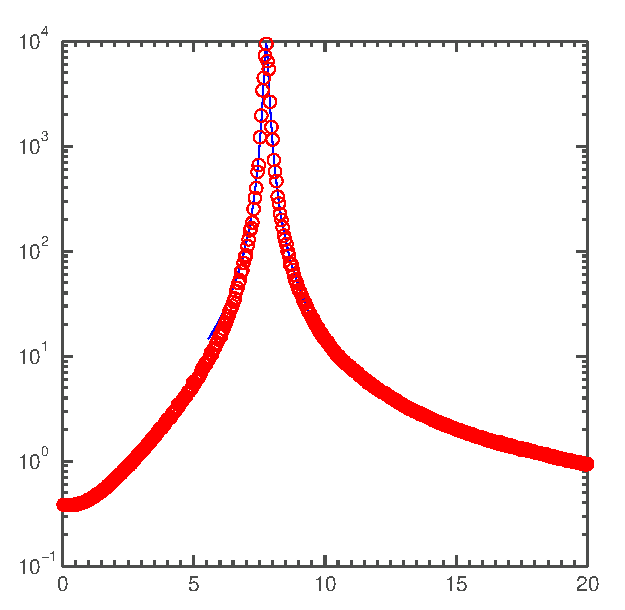
\includegraphics{sed.eps}}
\renewcommand{\figure}{Fig.}
\caption{Power spectra for selected modes of the $4\times 4$ perfect and mixed superlattices [indicated by the labeled gray square markers in Figs.~\ref{fig:dispersion}(a)-\ref{fig:dispersion}(c)]. Dark blue corresponds to a perfect superlattice, red corresponds to mixing of 80/20, and light blue corresponds to mixing of 60/40. Reported lifetimes calculated from the fitting of the Lorentzian functions (not shown) are also included. By removing a single MD seed, the average uncertainty in the fitting was determined to be 7.5\%.}
\label{fig:sed}
\end{center}
\end{figure*}
%%%

\subsection{Lifetimes}

The phonon lifetimes as a function of the harmonic frequencies are plotted in Fig.~\ref{FIG:lifetime}. As the period length increases, we maintain the same number of unit cells, such that the total number of atoms increases. Consequently, the minimum frequency decreases and the longest lifetime increases with increasing period length. Overall, the magnitudes of the lifetimes for a given frequency do not vary significantly from one superlattice to another. The lifetimes for all perfect superlattices exhibit $\omega^{-2}$ scaling at low frequencies. This result is consistent with theoretical predictions for phonon-phonon scattering of modes in the Debye regime, where the density of states scales as $\omega^{2}$ [see Fig.~\ref{fig:dispersion}(d)].\cite{Klemens_Thermal_1951} For the $8\times8$ and $14\times14$ superlattices, the perfect systems have two distinct trends that terminate at the maximum frequencies of the corresponding bulk systems (vertical lines in Fig.~\ref{FIG:lifetime}). The lifetimes in these two regions are comparable to the bulk lifetimes at the corresponding frequencies. This observation is consistent the emergence of bulk-like modes for the longer period superlattices as demonstrated by the PIPRs in Fig.~\ref{FIG:ipnum}.

Under the Debye approximation, a $\omega^{-4}$ lifetime scaling is predicted due to elastic phonon-point defect scattering.\cite{PhysRev.140.A1812,klemens_scattering_1955-3, klemens_thermal_1957-2} As mixing is introduced to the superlattices, a $\omega^{-4}$ scaling is observed at intermediate frequencies for the $2\times2$ and $4\times4$ superlattices but not for the $8\times8$ and $14\times14$ superlattices. The complicated dispersions of the superlattices, particularly for the $8\times8$ and $14\times14$ structures, where there is a significant amount of branch folding, are not Debye-like at the intermediate frequencies, leading to a deviation from the $\omega^{-4}$ scaling. The lifetimes of low-frequency modes for all mixed superlattices are not affected and follow a similar $\omega^{-2}$ scaling as seen in the perfect superlattices.

The introduction of interfacial mixing broadens the power spectra (Fig.~\ref{fig:sed}) and shifts the phonon lifetimes downward (Fig.~\ref{FIG:lifetime}), particularly at the intermediate and high frequencies. For the $2 \times 2$ and $ 4 \times 4$ mixed superlattices,  the lifetimes of some high-frequency modes fall below the Ioffe-Regel limit, $\tau_\mathrm{IR} =2\pi/\omega$, where a mode has a lifetime equal to its period of oscillation. The normal modes of a perfect superlattice have a plane wave structure. Under the assumption that the normal modes of a perfect superlattice are representative of the mixed superlattice, reaching the Ioffe-Regel limit is therefore not an indication of spatial localization but rather of temporal localization. This statement is supported by the inverse participation ratios, which, as shown in Fig.~\ref{fig:dispersion}(e), are all below the localization limit. Modes that are below the Ioffe-Regel limit can thus be considered to be non-propagating delocalized modes (i.e., diffusons).\cite{allen_thermal_1993,allen1999diffusons} A similar trend in the variation of lifetimes with frequency, dropping below the Ioffe-Regel limit at intermediate frequencies and then rising above at higher frequencies, has also been predicted for LJ alloys.\cite{larkin2013predicting} 

%%%
\renewcommand{\textfraction}{0.0}
\begin{figure}%[H!]
\begin{center}
\scalebox{1}{ \includegraphics{lifvomega.eps}}
\renewcommand{\figure}{Fig.}
\caption{Lifetimes for perfect (blue) and 80/20 (red) superlattices. The black line corresponds to the Ioffe-Regel criterion, $2\pi\omega^{-1}$. The brown line corresponds to $\omega^{-2}$ scaling. The green line corresponds to $\omega^{-4}$ scaling. Vertical grey lines correspond to the maximum frequency observed in the bulk systems: for the lighter species, $\omega_{m,max}=24.7$ and for the heavier species, $\omega_{3m,max}=14.3$. {\color{red}Lifetime is expressed in terms of the LJ potential parameters as $\tau=\tau^*\sqrt{\epsilon/\sigma^2m}$, where $\tau^*$ is the lifetime in units of seconds.} 
} 
\label{FIG:lifetime}
\end{center}
\end{figure}
%%%

\subsection{Thermal Conductivity}

\begin{table*}
\begin{center}
\begin{tabular*}{\textwidth}{c@{\extracolsep{\fill}}cccccc}
\hline\hline\noalign{\smallskip}
\multicolumn{2}{c}{\multirow{2}{*}{Cross-Plane}}& \multicolumn{4}{c}{$N\times N$ Superlattice} \\
\cline{3-6}\noalign{\smallskip}
\hspace{1cm} && $2\times2$ & $4\times4$ & $8\times8$ & $14\times14$  \\
\noalign{\smallskip}\hline\noalign{\smallskip}
\multirow{3}{*}{Perfect} &NMD & 0.29 $\pm$ 0.03 & 0.23 $\pm$ 0.02 & 0.32 $\pm$ 0.03 & 0.39 $\pm$ 0.04 \\
&GK & 0.25 $\pm$ 0.02 & 0.22 $\pm$ 0.02  &  0.29 $\pm$ 0.02  &  0.39 $\pm$ 0.03\\
&Thermal Circuit & 0.04  &  0.07  &  0.13  &  0.20\\
\noalign{\smallskip}\hline
\multirow{3}{*}{Mixed 80/20} &NMD &0.19 $\pm$ 0.02& 0.17 $\pm$ 0.02& 0.28 $\pm$ 0.03 & 0.42 $\pm$ 0.04\\
&GK  & 0.16 $\pm$ 0.01  &  0.18 $\pm$ 0.02 &  0.29 $\pm$ 0.02 &   0.45 $\pm$ 0.06\\
&Tamura (NMD) & 0.21 $\pm$ 0.02& 0.15 $\pm$ 0.02& 0.30 $\pm$ 0.03& 0.37 $\pm$ 0.04\\
\hline\hline
\end{tabular*}
\end{center}
\renewcommand{\table}{Table.}
\caption{Cross-plane thermal conductivity predictions [W/m-K].}
\label{TB:K_CP}
\end{table*}

\begin{table*}
\begin{center}
\begin{tabular*}{\textwidth}{c@{\extracolsep{\fill}}cccccc}
\hline\hline\noalign{\smallskip}
\multicolumn{2}{c}{\multirow{2}{*}{In-Plane}}&\multicolumn{4}{c}{$N\times N$ Superlattice} \\
\cline{3-6}\noalign{\smallskip}
\hspace{1cm} && $2\times2$ & $4\times4$ & $8\times8$ & $14\times14$  \\
\noalign{\smallskip}\hline\noalign{\smallskip}
\multirow{2}{*}{Perfect} &NMD &0.52 $\pm$ 0.05 & 0.51 $\pm$ 0.05& 0.56 $\pm$ 0.05& 0.60 $\pm$ 0.06\\
&GK &0.53 $\pm$ 0.03 &  0.54 $\pm$ 0.03 &  0.61 $\pm$ 0.05  &  0.66 $\pm$ 0.07 \\
&In-plane Diffuse Limit & 0.95 & 0.95 & 0.95 & 0.95\\
\noalign{\smallskip}\hline
\multirow{3}{*}{Mixed 80/20} & NMD &0.21 $\pm$ 0.02 & 0.25 $\pm$ 0.03 & 0.37 $\pm$ 0.04 & 0.47  $\pm$ 0.05\\
&GK & 0.19 $\pm$ 0.02 &  0.30 $\pm$ 0.01  & 0.43 $\pm$ 0.03 &  0.62 $\pm$ 0.07 \\   
&Tamura (NMD)& 0.22 $\pm$ 0.02 & 0.27 $\pm$ 0.03 & 0.38 $\pm$ 0.04 & 0.45 $\pm$ 0.05\\
\hline\hline
\end{tabular*}
\end{center}
\renewcommand{\table}{Table.}
\caption{In-plane thermal conductivity predictions [W/m-K].}
\label{TB:K_IP}
\end{table*}
%%%
\subsubsection{Perfect superlattices}
{\color{red}The GK method does not require assumptions about the nature of thermal transport or the types of modes present in the superlattices. As such, we consider the GK estimate of thermal conductivity to be a benchmark for comparison.} With reference to Tables~\ref{TB:K_CP} and~\ref{TB:K_IP}, the trends and magnitudes in cross-plane and in-plane thermal conductivity predictions from NMD and GK for perfect superlattices are in good agreement. Justification for the reported uncertainties is provided in Appendix~\ref{app:size effects}. The in-plane thermal conductivity increases with increasing period length, while the cross-plane thermal conductivity first decreases then increases with period length, consistent with previous MD superlattice studies.\cite {PhysRevB.77.184302,PhysRevB.72.174302} The in-plane thermal conductivity is nearly a factor of two larger than cross-plane thermal conductivity for all superlattices because of the larger group velocities across the entire frequency spectrum for the in-plane direction [see Figs.~\ref{fig:dispersion}(a) and~\ref{fig:dispersion}(c)]. 

A thermal circuit model prediction for cross-plane thermal conductivity using the relation\cite{PhysRevB.77.184302}
%%%
\begin{equation}\label{EQ:TCircuit}
\begin{split}
k_{CP,circuit}= \frac{La}{2R_{int}+\frac{La}{2k_m}+\frac{La}{2k_{3m}}},
\end{split}
\end{equation}
%%%
is presented in Table~\ref{TB:K_CP}. The boundary resistance for a perfect interface, estimated from the non-equilibrium direct method ($R_{int}=1.4\times10^{-8}$ Km$^2$W$^{-1}$),\cite{simonDM} was combined with bulk thermal conductivities, obtained from NMD, of the lighter material ($k_{m}$=1.2 W/m-K) and the heavier material ($k_{3m}$=0.7 W/m-K) through their respective layer thickness, yielding an effective resistance that was inverted to obtain an effective thermal conductivity. The thermal circuit model underestimates the thermal conductivity for all superlattices, indicating that the bulk phonons of the constituent species are not an accurate description of superlattice phonons. The relative difference decreases with increasing period length, however, suggesting that this model may become representative of the nature of thermal transport at large enough period lengths.
The diffusive limit for the in-plane direction, for superlattices with layers of equal length, is given by \cite{PhysRevB.77.184302}
%%%
\begin{equation}\label{EQ:TCircuit}
\begin{split}
k_{IP,diff}= \frac{k_m+k_{3m}}{2},
\end{split}
\end{equation}
%%%
is presented in Table~\ref{TB:K_IP}. The in-plane thermal conductivity predictions are expected to approach this limit as the superlattice period length is increased.

\subsubsection{Mixed superlattices}
From Tables~\ref{TB:K_CP} and~\ref{TB:K_IP}, the in-plane and cross-plane thermal conductivity predictions for the $2\times 2$ and $4\times 4$ mixed superlattices are reduced from their corresponding perfect system and approach the 50/50 alloy limit (0.21 W/m-K from GK using $N_{x,y,z}=6$). The mixed $2\times 2$ superlattice loses much of its anisotropy between the in-plane and cross-plane directions as there is mixing in all the atomic layers. From Table~\ref{TB:K_CP}, the cross-plane predictions for mixed superlattices from NMD (using perfect eigenvectors) and GK are in good agreement and follow similar trends, with increasing thermal conductivity with increasing period length. From Table~\ref{TB:K_IP}, for mixed superlattices, with the exception of  the $2 \times 2$ superlattice, NMD predicts a lower in-plane thermal conductivity than GK. The largest underprediction for the $14 \times 14$ superlattice is 25\%.

To shed light on the discrepancy between the GK and NMD in-plane predictions and to assess the assumption of using the perfect superlattice eigenvectors for the mixed superlattices, we also use Tamura elastic mass-defect scattering theory to predict thermal conductivities. \cite{tamura_isotope_1983,PhysRevB.87.140302,Luckyanova16112012} In this approach, the lifetimes predicted for perfect superlattices, $\tau_{perfect}\kv$, are modified using the Matthiesen rule 
%%%
\begin{equation}\label{EQ:tau_eff}
\begin{split}
\frac{1}{\tau_{effective}\kv} = \frac{1}{\tau_{perfect}\kv} +\frac{1}{\tau_{defect}\kv},
\end{split}
\end{equation}
%%%
where
%%%
\begin{equation}\label{EQ:tau_d}
\begin{split}
\frac{1}{\tau_{defect}\kv} = &\frac{\pi}{2N}\omega^2\kv \sum_{\pmb{\kappa'},\nu'} \left\{ \delta\left[ \omega\kv - \omega\kvp \right]
\left (\color{red} \sum_{b,\alpha} g_2(b) |e^*\kvbap e\kvba |^2 \right )\right \} .
\end{split}
\end{equation}
%%%
Here, $g_2(b)$ is the coupling term for atom $b$ in the unit cell that defines the strength of the mass disordering,
%%%
\begin{equation}\label{EQ:g(b)}
\begin{split}
g_2(b) = \sum_\mu c_{\mu}(b)\left[1-\frac{m_{\mu}(b)}{\overline{m(b)}}\right]^2, 
\end{split}
\end{equation}
%%%
where the summation is over the possible species at that atomic position in the unit cell with concentration $c_\mu(b)$, mass $m_\mu(b)$, and average mass $\overline{m(b)}$. Given that there are two atom types in the superlattice unit cell, the lighter atom can be considered to be a mass defect of the heavier portion of the superlattice, and vice-versa. $g_2(b)$ is zero if atom $b$ is unmixed (i.e., for atoms that do not reside within one monolayer of the interface). The delta function in Eq.~(\ref{EQ:tau_d}) is broadened into a Lorentzian function with width on the order of the frequency level spacing ($\approx 0.1$) imposed by the finite size of the systems.\cite{allen_thermal_1993}

The cross-plane and in-plane thermal conductivity predictions from NMD and Tamura theory are in good agreement, thus yielding a comparable discrepancy with the GK predictions for the in-plane thermal conductivity [see Table~\ref{TB:K_IP}]. While the discrepancy manifests in the in-plane direction, the effects occur at the mode level. This discrepancy is not observed for the cross-plane thermal conductivities because the most disrupted modes in the mixed superlattices (see Figs.~\ref{fig:sed} and~\ref{FIG:lifetime}) exist at intermediate frequencies that have a near-zero component of group velocity [Fig.~\ref{fig:dispersion}(a)]. The in-plane difference between NMD and Tamura theory with GK increases with period length because the number of branches with non-zero components of group velocity increases. The thermal conductivity predictions for the mixed superlattices indicate that the use of eigenvectors from perfect superlattices to represent modes in mixed superlattices in the NMD approach is equivalent to the perturbative approximation of Tamura theory. This perturbative approximation is not always valid for mixed superlattices, particularly for modes with a large density of states, where the most disruption is observed.

\section{Superlattice phonons}\label{SEC:sl_phon}
The term ``coherence" has been used in two contexts in relation to phonons. First, to describe the modes that emerge from a secondary periodicity (i.e., in a superlattice\cite{Luckyanova16112012}  or a thin film with a periodic arrangement of holes\cite{doi:10.1021/nl102918q,PhysRevB.87.195301}). Second, to describe the excitation of long-wavelength phonons, usually by femtosecond time-resolved pump-probe techniques,\cite{PhysRevLett.73.740,PhysRevB.75.195309} that do not carry significant thermal energy and are not found in the MD simulations studied here. The first context and its relation to thermal transport are the focus of this section.

In a crystalline solid, the phonons that carry thermal energy belong to the dispersion relation of that material, which depends on the geometry, the harmonic force constants, and the constituent masses. The introduction of a secondary periodicity modifies the dispersion such that modes emerge that do not exist in the composing bulk materials. These non-bulk phonons (in our case, superlattice phonons) propagate and scatter in the periodic structure in a similar manner to what a bulk phonon experiences in a bulk material. 

The existence of superlattice phonons has been argued based on modeling and experimental evidence. The predicted minimum in cross-plane thermal conductivity as a function of period length{\color{red}\cite{PhysRevB.66.024301,PhysRevB.77.184302,PhysRevB.67.195311,PhysRevB.72.174302,PhysRevB.61.3091,Imamura2003Lattice}} has been attributed to a transition of thermal transport dominated by superlattice phonons in short-period superlattices to thermal transport dominated by bulk-like phonons in longer-period superlattices.\cite{PhysRevLett.84.927,PhysRevB.56.10754} A thickness-dependent thermal conductivity of finite-size GaAs/AlAs superlattices measured experimentally was explained in terms of ballistic superlattice phonons.\cite{Luckyanova16112012} 

By using MD simulations, we do not impose any restrictions on the phonon dynamics. The system is allowed to move through its phase space naturally and thus all classical effects, including coherence and the emergence of superlattice phonons, should be captured. Our results indicate that using the superlattice normal modes captures the physics of thermal transport in a perfect superlattice, emphasizing the importance of using the correct dispersion relation. One cannot use the bulk material phonon properties to predict thermal transport in these non-bulk-like systems. This effect is clearly present for all the systems studied here, as evidenced by the discrepancy between the bulk-based thermal circuit model and the NMD and GK predictions (see Tables~\ref{TB:K_CP} and~\ref{TB:K_IP}). We note, however, that the PIPRs plotted in Fig. \ref{FIG:ipnum} suggest that lengthening the superlattice period length generates modes that are becoming localized to the individual layers.

As a means to study how superlattice phonons contribute to thermal conductivity, cross-plane and in-plane thermal conductivity accumulation functions are plotted in Fig.~\ref{FIG:MFP_cuml}. Also plotted are the accumulation functions for the two bulk species. The vertical coordinate of any point on the accumulation function represents the thermal conductivity that comes from phonons with MFPs less than the horizontal coordinate of that point.{\color{red}\cite{dames2005thermal}}

%%%
\begin{figure}%[H]
\begin{center}
\scalebox{1}{ \includegraphics{MFP_cp+ip_cuml_abs.eps}}
\renewcommand{\figure}{Fig.}
\caption{Thermal conductivity accumulation functions for bulk species and perfect and mixed superlattices.}
\label{FIG:MFP_cuml}
\end{center}
\end{figure}
%%%

The in-plane accumulation functions of the perfect and mixed superlattices exhibit asymptotic flattening at longer MFPs. The cross-plane accumulation functions of all superlattices contain step-like jumps at longer MFPs, a consequence of the the finite resolution of the Brillouin Zone.\cite{esfarjani2011heat} These longer MFPs correspond to the low-frequency modes that follow the $\omega^{-2}$ lifetime scaling [see Fig.~\ref{FIG:lifetime}] and have a non-zero group velocity component in the cross-plane direction [see Fig.~\ref{fig:dispersion}(a)]. The significant contributions of longer MFP modes in the cross-plane direction suggest a mechanism for reducing the cross-plane thermal conductivity through the finite size of thin-film superlattices.\cite{Luckyanova16112012} 

The majority of the contribution (greater than 90\%) to cross-plane thermal conductivity for all superlattices, perfect and mixed, is from modes with MFPs greater than the superlattice period length. Furthermore, 40\% ($2 \times 2 $) to 60\% ($14 \times 14$) of cross-plane and in-plane conductivity is from modes with MFPs greater than the system size in those directions ($N_xLa$ for the cross-plane and $N_ya$ for the in-plane). For the bulk materials, the entire contribution to thermal conductivity comes from modes with MFPs greater than the lattice constant, with 50\% of the contribution from modes with MFPs greater than the system length. {\color{red} MFPs can be larger than the MD system size because the lifetime for an individual phonon mode is fundamental quantity that represents the time it takes for the energy in a mode to become uncorrelated. \cite{PhysRevB.71.184305} As such, the determination of the lifetime does not require the manifestation of the MFP, which is calculated using Eq.~(\ref{EQ:M:phonon_mfp}), in the MD system.} In the perfect superlattices, MFPs greater than the period length cannot be interpreted any differently than MFPs greater than the lattice constant of a bulk crystalline structure. Based on the accumulation functions and good agreement with GK thermal conductivity predictions, our results indicate that, for the range of superlattices studied here, perfect superlattice phonons and bulk phonons can be treated in the same theoretical frameworks. In this case, the concept of coherent effects can be argued to be purely interpretational and is not required to model phonon transport in these superlattices. 

Mixing shifts the in-plane thermal conductivity contribution to shorter MFPs for the $2 \times 2 $ and $4 \times 4 $ superlattices. Differences between perfect and mixed accumulations functions for cross-plane thermal conductivity manifest at intermediate and longer MFPs. These differences for the in-plane and cross-plane, however, become increasingly smaller with increasing period length. Furthermore, mixing does not change the range of MFPs. While the perfect and mixed accumulation functions share similar trends, the discrepancy between the NMD and GK in-plane thermal conductivity predictions indicates that some of the mixed modes are fundamentally different than the those of the perfect superlattices. The modes in the mixed superlattices cannot be perfectly described by the modes of perfect superlattices and, therefore, the mixed in-plane accumulation functions are not complete representations of the thermal conductivity.

\section{Summary}

We used NMD to predict phonon properties at 20 K in perfect and mixed LJ superlattices with a mass ratio of three. Differences between in-plane and cross-plane components of group velocity are responsible for the differences between in-plane and cross-plane thermal conductivities [Figs.~\ref{fig:dispersion}(a)-(c), Tables ~\ref{TB:K_CP} and ~\ref{TB:K_IP}]. By fitting the mode power spectra to Lorentzian lineshapes, we observe a $\omega^{-2}$ lifetime scaling for low-frequency modes in perfect and mixed superlattices in Fig.~\ref{FIG:lifetime}. In longer period-length perfect superlattices ($8 \times 8$ and $14 \times 14$), two distinct lifetime trends that terminate at the maximum bulk frequencies were attributed to the separation in the participation of these modes in the layers of the superlattice [see Fig.~\ref{FIG:ipnum}]. In mixed superlattices, these trends become smeared and a $\omega^{-4}$ lifetime scaling emerges at intermediate frequencies in the $2 \times 2$ and $4 \times 4$ superlattices, indicating elastic mass point defect scattering of Debye-like phonons. We find that interspecies mixing disrupts the secondary periodicity [see panel B in Fig.~\ref{fig:sed}] and reduces phonon lifetimes, manifesting in a discrepancy between the in-plane thermal conductivity predictions for mixed superlattices from GK with NMD and Tamura theory [see Table~\ref{TB:K_IP}]. The discrepancy is the consequence of the use of eigenvectors from perfect superlattices to describe the modes in mixed superlattices.

Our results demonstrate that further effort is required in order to improve our understanding of the effects of mixing on superlattice phonons. A crucial step is obtaining detailed experimental characterization of the quality of these interfaces, which can then be used as input into the modeling frameworks presented here. Due to the computational cost of DFT-based approaches, MD simulation will continue to be a valuable tool in establishing models of phonon transport in superlattices where the perturbative approach to mixing breaks down.

\section{Acknowledgements}
SCH and CHA acknowledge the support of OGS, NSERC, and AMD. JML and AJHM acknowledge the support from NSF award DMR1006480. We thank Simon Lu, (Carnegie Mellon University), for performing the direct method simulations of the isolated interface thermal resistance.

\newpage
\appendix
\section{Size effects}\label{app:size effects}
Due to their large unit cells, mode-by-mode studies of superlattices are computationally expensive and accounting for size effects in thermal conductivity prediction is challenging. For example, Broido \textit{et al}. were limited to a maximum period length of $8\times 8$ using an iterative solution to the BTE for Si/Ge.\cite {PhysRevB.70.081310} In other studies, the phonon properties for short period Si/Ge superlattices obtained from DFPT were presumed to hold for larger period superlattices.\cite{Luckyanova16112012, doi:10.1021/nl202186y} Similarly, Savic \textit{et al.} extrapolate the phonon lifetimes of low frequency modes of Si/Ge superlattices from a power law fitted to data obtained from a Monte Carlo integration of the BTE.\cite{savic:073113} 

A comparison of the thermal conductivity predictions for superlattices with different system sizes is presented in Tables~\ref{TB:K_CP_NMDsize} (cross-plane) and~\ref{TB:K_IP_NMDsize} (in-plane). The NMD predictions for both the cross-plane and in-plane thermal conductivities varied by 10\% when increasing $N_x$ from six to eight along the cross-plane and fixing $N_y$ and $N_z$ at six ($N_x$ was set to ten for the $2\times2$ superlattices to resolve the lifetime scalings). Due to the scaling of the NMD algorithm [$O(N_xN_yN_z L)$], further increasing the Brillouin zone resolution ($N_i$) was computationally prohibitive. As a result of these size effects, the reported thermal conductivity predictions from NMD are presumed to carry an uncertainty of 10\%. Uncertainty in the GK prediction was specified by systematically removing one seed before calculating the thermal conductivity.

We note that one approach to estimating size effects in NMD thermal conductivity predicitions is to conduct simulations for a range of system sizes, plot the inverse of thermal conductivity versus the inverse of the system length, fit a line through the data, and then take the vertical axis intercept as the bulk value.\cite{PhysRevB.81.214305} This method was not used in previous superlattice studies \cite{doi:10.1021/nl202186y,savic:073113,Luckyanova16112012} and is not used here. The complicated dispersion [Figs.~\ref{fig:dispersion}(a)-(c)] does not guarantee that this approach is valid and, as such, understanding size effects in superlattices warrants further work.

\begin{table*}[h!]
\begin{center}
\begin{tabular*}{\textwidth}{c@{\extracolsep{\fill}}ccccc}
\hline\hline\noalign{\smallskip}
Cross-Plane Perfect& \multicolumn{4}{c}{Superlattice} \\
\cline{2-5}\noalign{\smallskip}
$N_x\times N_y \times N_z$ & $2\times2$ & $4\times4$ & $8\times8$ & $14\times14$  \\
\noalign{\smallskip}\hline\noalign{\smallskip}
$6\times6\times6$ & 0.23  & 0.22  &  0.28  &  0.36 \\
$8\times6\times6$ & 0.28  & 0.23  &  0.32  &  0.39 \\
$10\times6\times6$ & 0.29  &  - &  -  &  - \\
\hline\hline
\end{tabular*}
\end{center}
\renewcommand{\table}{Table.}
\caption{Size-dependent cross-plane NMD predictions of thermal conductivity [W/m-K].}
\label{TB:K_CP_NMDsize}
\end{table*}

\begin{table*}[h!]
\begin{center}
\begin{tabular*}{\textwidth}{c@{\extracolsep{\fill}}ccccc}
\hline\hline\noalign{\smallskip}
In-Plane Perfect& \multicolumn{4}{c}{Superlattice} \\
\cline{2-5}\noalign{\smallskip}
$N_x\times N_y \times N_z$ & $2\times2$ & $4\times4$ & $8\times8$ & $14\times14$  \\
\noalign{\smallskip}\hline\noalign{\smallskip}
$6\times6\times6$ & 0.53 & 0.51  &  0.56  &  0.59 \\
$8\times6\times6$ & 0.52 & 0.51  &  0.55  &  0.58 \\
$10\times6\times6$ & 0.52 & -  &  -  &  - \\
\hline\hline
\end{tabular*}
\end{center}
\renewcommand{\table}{Table.}
\caption{Size-dependent in-plane NMD predictions of thermal conductivity [W/m-K].}
\label{TB:K_IP_NMDsize}
\end{table*}

\newpage
\bibliographystyle{apsrev}
\bibliography{superlattice.bib}

\end{document}

